\documentclass[conference,a4paper]{IEEEtran}
\IEEEoverridecommandlockouts
\usepackage[T1]{fontenc}
\usepackage[utf8]{inputenc}
\usepackage{microtype}
\usepackage{cite}
\usepackage{amsmath,amssymb,amsfonts}
\usepackage{graphicx}
\usepackage{textcomp}
\usepackage{booktabs}
\usepackage{array}
\usepackage{tabularx}
\usepackage{xcolor}
\usepackage{bm}
\usepackage{hyperref}
\usepackage[caption=false,font=footnotesize]{subfig}
\usepackage{cleveref}

\definecolor{PaperLinkBlue}{HTML}{0057FF}
\definecolor{NeonRefGreen}{HTML}{39FF14}
\hypersetup{
  colorlinks=true,
  linkcolor=PaperLinkBlue,
  urlcolor=PaperLinkBlue,
  filecolor=PaperLinkBlue,
  citecolor=NeonRefGreen,
  pdfauthor={Anonymous Authors},
  pdftitle={Mapping Quantum Reservoir Advantage},
  pdfsubject={Quantum reservoir computing, time-series forecasting, benchmark atlas, echo state networks}
}

\renewcommand{\tableautorefname}{Tab.}
\renewcommand{\figureautorefname}{Fig.}
\graphicspath{{gfx/}}
\setlength{\textfloatsep}{8pt plus 2pt minus 2pt}
\setlength{\floatsep}{7pt plus 2pt minus 2pt}
\setlength{\intextsep}{7pt plus 2pt minus 2pt}
\interdisplaylinepenalty=2500
\raggedbottom

\newcommand{\qrc}{\mathrm{QRC}}
\newcommand{\esn}{\mathrm{ESN}}
\newcommand{\nrmse}{\mathrm{NRMSE}}
\newcommand{\mae}{\mathrm{MAE}}
\newcommand{\R}{\mathbb{R}}
\newcommand{\Tr}{\operatorname{Tr}}

\begin{document}

\title{Mapping Quantum Reservoir Advantage}

\author{%
\IEEEauthorblockN{Anonymous Authors}
\IEEEauthorblockA{Anonymous submission}
}
\maketitle
\thispagestyle{empty}
\pagestyle{empty}

\begin{abstract}
Quantum reservoir computing is often evaluated as a direct forecasting competitor to classical reservoirs. For practitioners, the sharper question is conditional: which datasets make a quantum reservoir worth testing? We present a dataset-regime benchmark comparing globally frozen QRC protocols against a feature-matched echo state network. Each dataset is described by measured time-series properties, and a meta-model maps those properties to empirical QRC usefulness. The result is not broad average superiority. The clearest QRC-favorable regime is slow, stateful forecasting: drifting trends, persistent low-frequency structure, regime changes, and temporally correlated fluctuations. The benchmark reframes quantum reservoir advantage as dataset-level triage.

\end{abstract}

\begin{IEEEkeywords}
quantum reservoir computing, echo state networks, time-series forecasting, benchmark atlas, quantum advantage triage
\end{IEEEkeywords}

\section{Introduction}
\label{sec:introduction}
Quantum reservoir computing follows a simple hybrid-learning pattern: fixed quantum dynamics transform an input stream into measured expectation-value features, and only a classical readout is trained~\cite{fujii2017harnessing,nakajima2019boosting,ghosh2019quantum}. This makes QRC attractive for near-term time-series forecasting because the quantum component is not variationally optimized. The open benchmark question is different from the hardware-scaling question: \emph{given a new dataset, when is a quantum reservoir worth trying against a strong classical reservoir?}

We answer this question empirically through a large dataset-regime atlas. We use ``quantum reservoir advantage'' in a deliberately scoped sense: a frozen QRC protocol has lower test error than a frozen feature-matched ESN on the same forecasting task. This is not a complexity-theoretic quantum-advantage claim. It is a benchmark claim about which dataset regimes favor a fixed quantum reservoir feature map over a canonical ESN feature map.

The central result is selective rather than universal. Across the held-out validation split, the best frozen QRC variant beats the ESN in 32.4\% of datasets and is clearly useful in 12.5\%. The mean best-QRC advantage is negative, so the ESN remains the stronger default. Yet the QRC wins are not noise. They recur across independent discovery and validation splits and are predictable from precomputed dataset descriptors. A meta-model trained on discovery rows distinguishes QRC-useful validation cases with ROC-AUC 0.836 and PR-AUC 0.431, more than three times the 12.5\% base useful rate.

This changes the practical question. Instead of asking whether QRC is generally better than ESNs, the atlas asks whether a dataset lies in a QRC-favorable regime. The strongest and most reproducible regime in the present benchmark is slow, stateful temporal structure: drifting trends, regime changes, persistent low-frequency components, long memory, and temporally correlated fluctuations. The useful regions are not summarized by one scalar descriptor. They arise from interactions among trend strength, spectral structure, persistence, volatility memory, predictability, and nonstationarity.

Our contributions are:
\begin{itemize}
    \item \textbf{A frozen-protocol atlas for empirical quantum reservoir advantage:} we build a 50,000-row property candidate atlas and evaluate 20,000 labeled discovery/validation datasets from 52 base generators and 16 broad time-series families under globally calibrated, then frozen, QRC and ESN protocols.
    \item \textbf{Selective advantage, not average superiority:} the ESN remains the stronger default, but QRC wins form reproducible pockets rather than isolated outliers.
    \item \textbf{The strongest QRC-usefulness regime:} the clearest favorable region is slow, stateful forecasting with drifting trends, regime changes, persistent low-frequency structure, long memory, and correlated fluctuations.
    \item \textbf{Dataset-level quantum-advantage triage:} measured dataset properties predict where QRC is worth testing before a practitioner pays the cost of running a quantum reservoir; the released artifact includes a CSV triage CLI for new univariate series.
    \item \textbf{Mechanism-resolved benchmark evidence:} separate frozen QRC variants distinguish reservoir-dynamics, reuploading, and dissipative protocols without turning the result into per-dataset tuning.
\end{itemize}


\section{Preliminaries}
\label{sec:background}
We formalize QRC and ESN forecasting as fixed feature-map comparisons with a trained readout. For a univariate or input-driven time series, a reservoir maps the history up to time \(t\) into a feature vector \(\Phi_t\in\R^D\). The readout is fit on a training split and evaluated on a held-out test split. The primary error metric is normalized root mean squared error,
\begin{equation}
    \nrmse =
    \frac{\sqrt{\frac{1}{T}\sum_t (y_t-\hat y_t)^2}}
    {\operatorname{std}(y_t)} .
    \label{eq:nrmse}
\end{equation}

\subsection{QRC as a fixed measured feature map}

For QRC, the feature map is generated by fixed quantum dynamics. Given input \(u_t\), the reservoir state evolves under an input-dependent quantum channel
\begin{equation}
    \rho_t = \mathcal{Q}_{u_t}(\rho_{t-1}),
    \qquad
    \Phi_t =
    \big(\Tr[O_a\rho_t]\big)_{a=1}^{D},
    \label{eq:qrc-feature}
\end{equation}
where \(O_a\) are measured observables. Only the classical readout is trained. In the v5 protocol, the QRC family consists of three canonical frozen variants: a mechanistic disordered spin-QRC (QRC-M), an encoding-enhanced variant with fixed reuploading (QRC-E), and a mildly dissipative variant (QRC-D). All use the same feature dimension as the ESN comparator.

\subsection{ESN comparator}

Echo state networks are the classical reservoir-computing baseline most directly matched to QRC: random recurrent dynamics produce a nonlinear state, and only the readout is trained~\cite{jaeger2004harnessing,lukosevicius2009reservoir}. Our ESN is a sparse random leaky reservoir with globally calibrated spectral radius, leak rate, and input scale. Its reservoir size is matched to the QRC feature dimension. This makes the comparison a fixed quantum feature map versus a fixed classical recurrent feature map, not a per-dataset tuning contest.

\subsection{Dataset-regime view}

The atlas treats QRC advantage as a property of a dataset regime. For each dataset \(i\), define
\begin{equation}
    A_i =
    \nrmse_{\esn,i}
    -
    \min_{v\in\{\mathrm{M,E,D}\}}\nrmse_{\qrc_v,i}.
    \label{eq:advantage}
\end{equation}
Positive \(A_i\) means that the best frozen QRC variant beats the frozen ESN. We call a case \emph{useful} when \(A_i\geq 0.05\). The meta-model then asks whether measured descriptors \(z_i\) predict the label \(A_i\geq 0.05\) before running the QRC.


\section{Related Work}
\label{sec:relatedwork}
Reservoir computing was introduced to exploit high-dimensional recurrent dynamics while training only a simple readout~\cite{maass2002real,jaeger2004harnessing,lukosevicius2009reservoir}. ESNs remain the most direct classical comparator for QRC because they share the same learning structure: fixed recurrent dynamics, nonlinear temporal features, and a trained linear readout. NVAR provides an important fixed-feature robustness baseline for nonlinear forecasting, but it is not the closest reservoir-to-reservoir comparison~\cite{gauthier2021next}.

QRC transfers this architecture to quantum dynamics. Disordered spin ensembles, spatial multiplexing, and driven quantum systems have been proposed as fixed temporal feature maps~\cite{fujii2017harnessing,nakajima2019boosting,ghosh2019quantum}. More recent work shows why protocol details matter: spin-network performance depends on dynamical regimes~\cite{martinezpena2021dynamical}, dissipation can be an active resource rather than a nuisance~\cite{sannia2024dissipation}, and input encoding can itself provide strong nonlinear transformations~\cite{govia2022nonlinear}. These results motivate our split between mechanistic, encoding-enhanced, and dissipative QRC variants.

Time-series benchmark archives and forecasting competitions show that model ranking is strongly dataset-dependent: seasonality, persistence, noise, nonstationarity, and regime changes can dominate average scores~\cite{makridakis2018m4,godahewa2021monash}. Our contribution is to connect this dataset-regime view to QRC. Rather than reporting only a mean QRC-versus-ESN score, we measure dataset properties, label empirical advantage under a frozen protocol, and learn where in property space QRC becomes useful.

The paper is therefore complementary to mechanism studies. It identifies \emph{where} QRC is empirically worth testing under a controlled benchmark. It does not prove \emph{why} those regimes arise from a particular quantum mechanism.


\section{Methodology}
\label{sec:methodology}
The benchmark is designed to avoid two common confounds: per-dataset reservoir tuning and post-hoc model selection. We calibrate QRC and ESN hyperparameters once on held-out synthetic calibration datasets, then freeze them for the atlas evaluation.

\subsection{Frozen QRC variants}

All QRC variants use a six-qubit disordered transverse-field spin reservoir with complete coupling topology, five internal layers, and three virtual nodes, giving 63 measured features. QRC-M uses input injection without repeated reuploading or dissipation. QRC-E uses the same reservoir with fixed input reuploading, motivated by practical QRC feature-map protocols and by the need to expose encoding contributions explicitly~\cite{govia2022nonlinear}. QRC-D uses the same reservoir with mild local dissipation, reflecting the current view that dissipation can be a useful design axis in QRC~\cite{sannia2024dissipation}. Calibration selects one global setting per variant: QRC-M uses \(J=1.5, dt=0.25\), QRC-E uses \(J=1.0, dt=0.25\), and QRC-D uses \(J=1.0, dt=0.15\) with mild damping.

\begin{table}[!t]
\centering
\caption{Frozen reservoirs used in the benchmark. All reservoirs are calibrated once, then reused without per-dataset tuning.}
\label{tab:reservoir-protocols}
\scriptsize
\setlength{\tabcolsep}{3.0pt}
\renewcommand{\arraystretch}{1.05}
\begin{tabularx}{\columnwidth}{@{}lXc@{}}
\toprule
Model & Role in the paper & Dim. \\
\midrule
QRC-M & Mechanistic spin-QRC with input injection only. Tests the fixed coupled reservoir dynamics with minimal extra encoding. & 63 \\
QRC-E & Same spin reservoir with fixed repeated input reuploading. Tests a practical encoding-enhanced QRC feature map. & 63 \\
QRC-D & Same spin reservoir with mild dissipation. Tests a realistic open-system QRC design axis. & 63 \\
ESN & Sparse random leaky ESN with globally calibrated spectral radius, leak, and input scale. Primary classical comparator. & 63 \\
\bottomrule
\end{tabularx}
\end{table}

\subsection{Frozen ESN comparator}

The ESN is a canonical sparse random leaky reservoir with the same feature dimension as QRC. The global calibration selects spectral radius 0.7, leak 0.3, and input scale 0.3. Once selected, the ESN is frozen for every atlas row. This ensures that the benchmark measures dataset-regime sensitivity rather than per-dataset reservoir optimization.

The ESN is intentionally the primary comparator because it is the closest classical analogue of QRC: both models use fixed recurrent dynamics and train only a linear readout. Linear ridge, gradient boosting, and NVAR are retained as contextual baselines, but the headline label is always QRC versus ESN. This keeps the title claim narrow: the paper maps empirical QRC advantage relative to the traditional reservoir-computing baseline, not relative to every possible forecasting method.

\subsection{Dataset descriptors and meta-model}

Each dataset is profiled by 30 Tier-A descriptors. The original 20 core descriptors include autocorrelation time, mutual-information minimum, memory capacity, linear predictability, nonlinear-gain contrast, signal-to-noise ratio, Lyapunov and 0--1 chaos diagnostics, spectral entropy, dominant frequency, stationarity tests, differencing order, scaling exponents, permutation/sample entropy, Hurst estimate, forecastability, and GBM predictability. Ten additional descriptors capture predictability gaps, volatility memory, ARCH structure, recurrence, spectral slope/centroid, trend strength, changepoints, and Lempel--Ziv complexity.

The descriptors are organized into six interpretable blocks: memory and persistence; predictability; spectrum and oscillation; nonstationarity and drift; noise and volatility; and nonlinear, chaotic, entropy, and recurrence structure. The blocks are intentionally redundant at the measurement level. For example, slow structure can appear as a high autocorrelation timescale, a large scaling exponent, low spectral centroid, strong trend score, or a stationarity-test signal. The meta-model is allowed to combine these partially overlapping views, while the ablation suite checks that the result is not carried by one proxy family.

The meta-model is trained only on discovery rows and evaluated once on validation rows. It uses gradient-boosted trees for regression on \(A_i\) and classification of \(A_i\geq 0.05\). We report ROC-AUC and PR-AUC because useful QRC cases are rare. Feature-set ablations test whether the signal survives after removing direct predictability proxies or restricting to persistence/spectral/nonstationarity descriptors.

\subsection{Quantum-advantage triage}

The output is a triage map, not a universal model ranking. Given a new dataset, the practitioner measures the descriptors \(z_i\), locates the dataset in the atlas, and estimates whether QRC is worth testing. We call this \emph{dataset-level quantum-advantage triage}: identifying plausible empirical QRC advantage before investing in quantum-reservoir evaluation.


\section{Experimental Setup}
\label{sec:experimental}
The v5 atlas contains 20,000 labeled datasets split into 10,000 discovery and 10,000 validation rows. They are selected from a 50,000-row candidate pool and span 52 base generators grouped into 16 broad families. The families include chaotic maps and flows, input-driven memory systems, oscillatory and quasiperiodic systems, long-range processes, colored noise, drifting trends, regime switching, seasonal/calendar structure, volatility-heteroskedastic processes, delay dynamics, intermittent sparse processes, nonlinear autoregressions, heavy-tail jumps, and multiscale composites.

The 50,000-row candidate pool is used to make the final atlas broad without turning the paper into an unstructured random sweep. Candidate series are first generated across the full taxonomy with varied seeds and parameters. The final discovery and validation rows are then selected to cover both broad family balance and frontier enrichment near the regions where QRC and ESN are close. This matters scientifically: a purely average benchmark would mostly estimate that ESN is the stronger default, whereas a regime atlas must also contain enough near-boundary and QRC-favorable examples to learn where the boundary lies.

\begin{table}[!t]
\centering
\caption{Frozen v5 protocol and held-out validation summary.}
\label{tab:v5-summary}
\footnotesize
\setlength{\tabcolsep}{3.0pt}
\renewcommand{\arraystretch}{1.03}
\begin{tabularx}{\columnwidth}{@{}lX@{}}
\toprule
Item & Value \\
\midrule
Discovery / validation rows & 10,000 / 10,000 \\
Families / base generators & 16 / 52 \\
Measured descriptors & 30 Tier-A properties \\
QRC variants & QRC-M, QRC-E, QRC-D \\
Feature dimension & 63 for QRC and ESN \\
Best-QRC win rate & 32.4\% on validation \\
Best-QRC useful rate & 12.5\% on validation \\
Mean best-QRC advantage & \(-0.058\) on validation \\
\bottomrule
\end{tabularx}
\end{table}

The target is one-step or short-horizon forecasting with train/validation/test splits derived from each generated series. All preprocessing is fit on training data only. The v5 evaluation records NRMSE and NMAE for linear ridge, gradient boosting, NVAR, the frozen ESN, and all three QRC variants. The primary label is the NRMSE advantage of the best QRC variant over the ESN. We also retain variant-specific advantages so that the atlas can distinguish whether QRC-M, QRC-E, or QRC-D is responsible for a QRC-favorable row.

\begin{table}[!t]
\centering
\caption{Descriptor blocks used for the 30-feature regime map.}
\label{tab:feature-blocks}
\scriptsize
\setlength{\tabcolsep}{3.0pt}
\renewcommand{\arraystretch}{1.05}
\begin{tabularx}{\columnwidth}{@{}lX@{}}
\toprule
Block & Examples \\
\midrule
Memory and persistence & Autocorrelation time, memory capacity, DFA exponent, Hurst estimate \\
Predictability & Linear and GBM NRMSE, nonlinear-gain contrast, predictability gap \\
Spectrum & Spectral entropy, flatness, dominant frequency, spectral slope and centroid \\
Drift and stationarity & ADF/KPSS signals, differencing order, trend strength, changepoints \\
Noise and volatility & SNR, volatility autocorrelation, ARCH statistic \\
Nonlinear structure & Lyapunov estimate, 0--1 statistic, entropy, recurrence, Lempel--Ziv complexity \\
\bottomrule
\end{tabularx}
\end{table}

NRMSE is the primary metric because it is scale-free and standard for forecasting comparisons. NMAE is recorded as a robustness metric because it is less sensitive to rare large errors. The main paper uses NRMSE labels; the artifact tables preserve NMAE columns for follow-up robustness checks and for readers who prefer absolute-error normalization.

The paper-facing analysis package writes all tables and figures from the completed v5 outputs. The main validation outputs are the complete validation table, the split/family/variant summaries, the discovery-trained validation predictions, the feature-set robustness table, and the rule-pocket table. All reported numbers in this paper are taken from these generated artifacts.


\section{Evaluation}
\label{sec:evaluation}
The evaluation is organized around the five paper claims: selectivity, predictability, slow-stateful regimes, interacting descriptors, and dataset-level triage.

\begin{figure*}[!t]
    \centering
    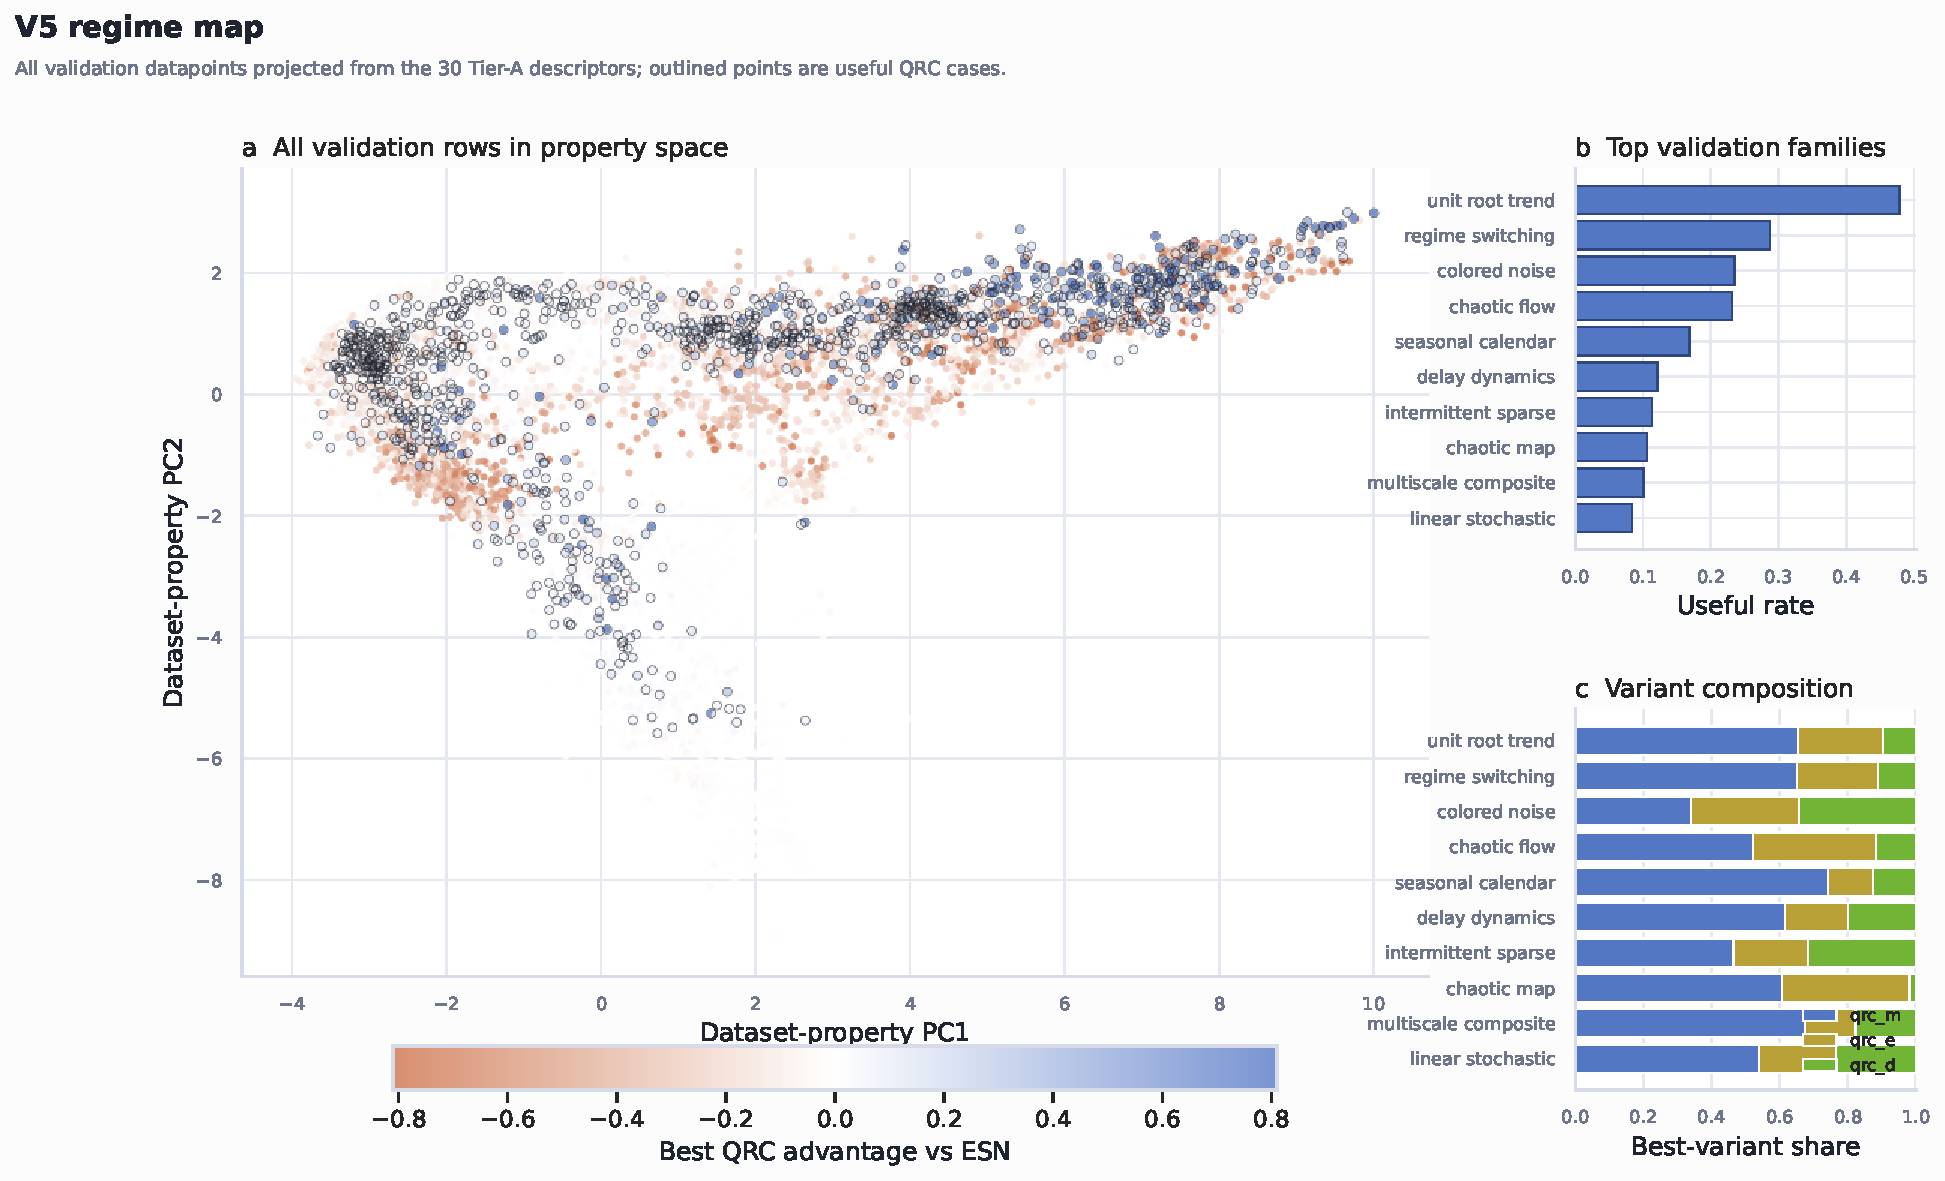
\includegraphics[width=0.88\textwidth]{regime-map.pdf}
    \caption{Validation regime map. Each point is one synthetic time-series dataset projected from 30 measured descriptors. Color denotes best-QRC advantage over the frozen ESN; outlined points meet the useful threshold. The side panels summarize the families where QRC is most often useful and which QRC variant is selected.}
    \label{fig:regime-map}
\end{figure*}

\subsection{QRC is selective, not broadly dominant}

QRC does not win on average. In validation, the mean ESN NRMSE is 0.805 and the mean best-QRC NRMSE is 0.863, giving mean best-QRC advantage \(-0.058\). However, QRC wins are not random leftovers: the best frozen QRC variant beats the ESN in 32.4\% of validation rows and reaches the useful threshold in 12.5\%. Discovery is similar, with 32.6\% win rate and 11.8\% useful rate. This discovery/validation agreement supports the first claim: empirical quantum reservoir advantage is selective but reproducible.

\begin{table}[!t]
\centering
\caption{Validation performance by frozen model. Advantage is measured against the frozen ESN.}
\label{tab:baseline-summary}
\scriptsize
\setlength{\tabcolsep}{3.4pt}
\renewcommand{\arraystretch}{1.05}
\begin{tabular}{lrrrr}
\toprule
Model & Mean NRMSE & Median & Win & Mean adv. \\
\midrule
Linear ridge & 0.802 & 0.945 & 47.5 & +0.003 \\
GBM & 0.782 & 0.907 & 39.3 & +0.023 \\
NVAR & 0.844 & 0.962 & 35.3 & -0.039 \\
Frozen ESN & 0.805 & 0.919 & -- & 0.000 \\
Best QRC & 0.863 & 0.959 & 32.4 & -0.058 \\
\bottomrule
\end{tabular}
\end{table}

\begin{table}[!t]
\centering
\caption{Validation performance by frozen QRC variant.}
\label{tab:variant-summary}
\scriptsize
\setlength{\tabcolsep}{3.5pt}
\renewcommand{\arraystretch}{1.04}
\begin{tabular}{lrrrr}
\toprule
Variant & Mean adv. & Median adv. & Win & Useful \\
\midrule
QRC-M dynamics & -0.100 & -0.029 & 22.0 & 9.4 \\
QRC-E reupload & -0.155 & -0.058 & 16.2 & 6.9 \\
QRC-D dissipative & -0.239 & -0.090 & 14.0 & 5.5 \\
Best QRC & -0.058 & -0.011 & 32.4 & 12.5 \\
\bottomrule
\end{tabular}
\end{table}

The best-QRC row is not per-dataset tuning. It is the best member of a small, fixed menu of canonical QRC protocols. The interpretation is practical: if a user is willing to test a few defensible QRC mechanisms, the atlas asks where at least one is useful against the same frozen ESN.

\subsection{Dataset properties predict QRC usefulness}

\begin{figure*}[!t]
    \centering
    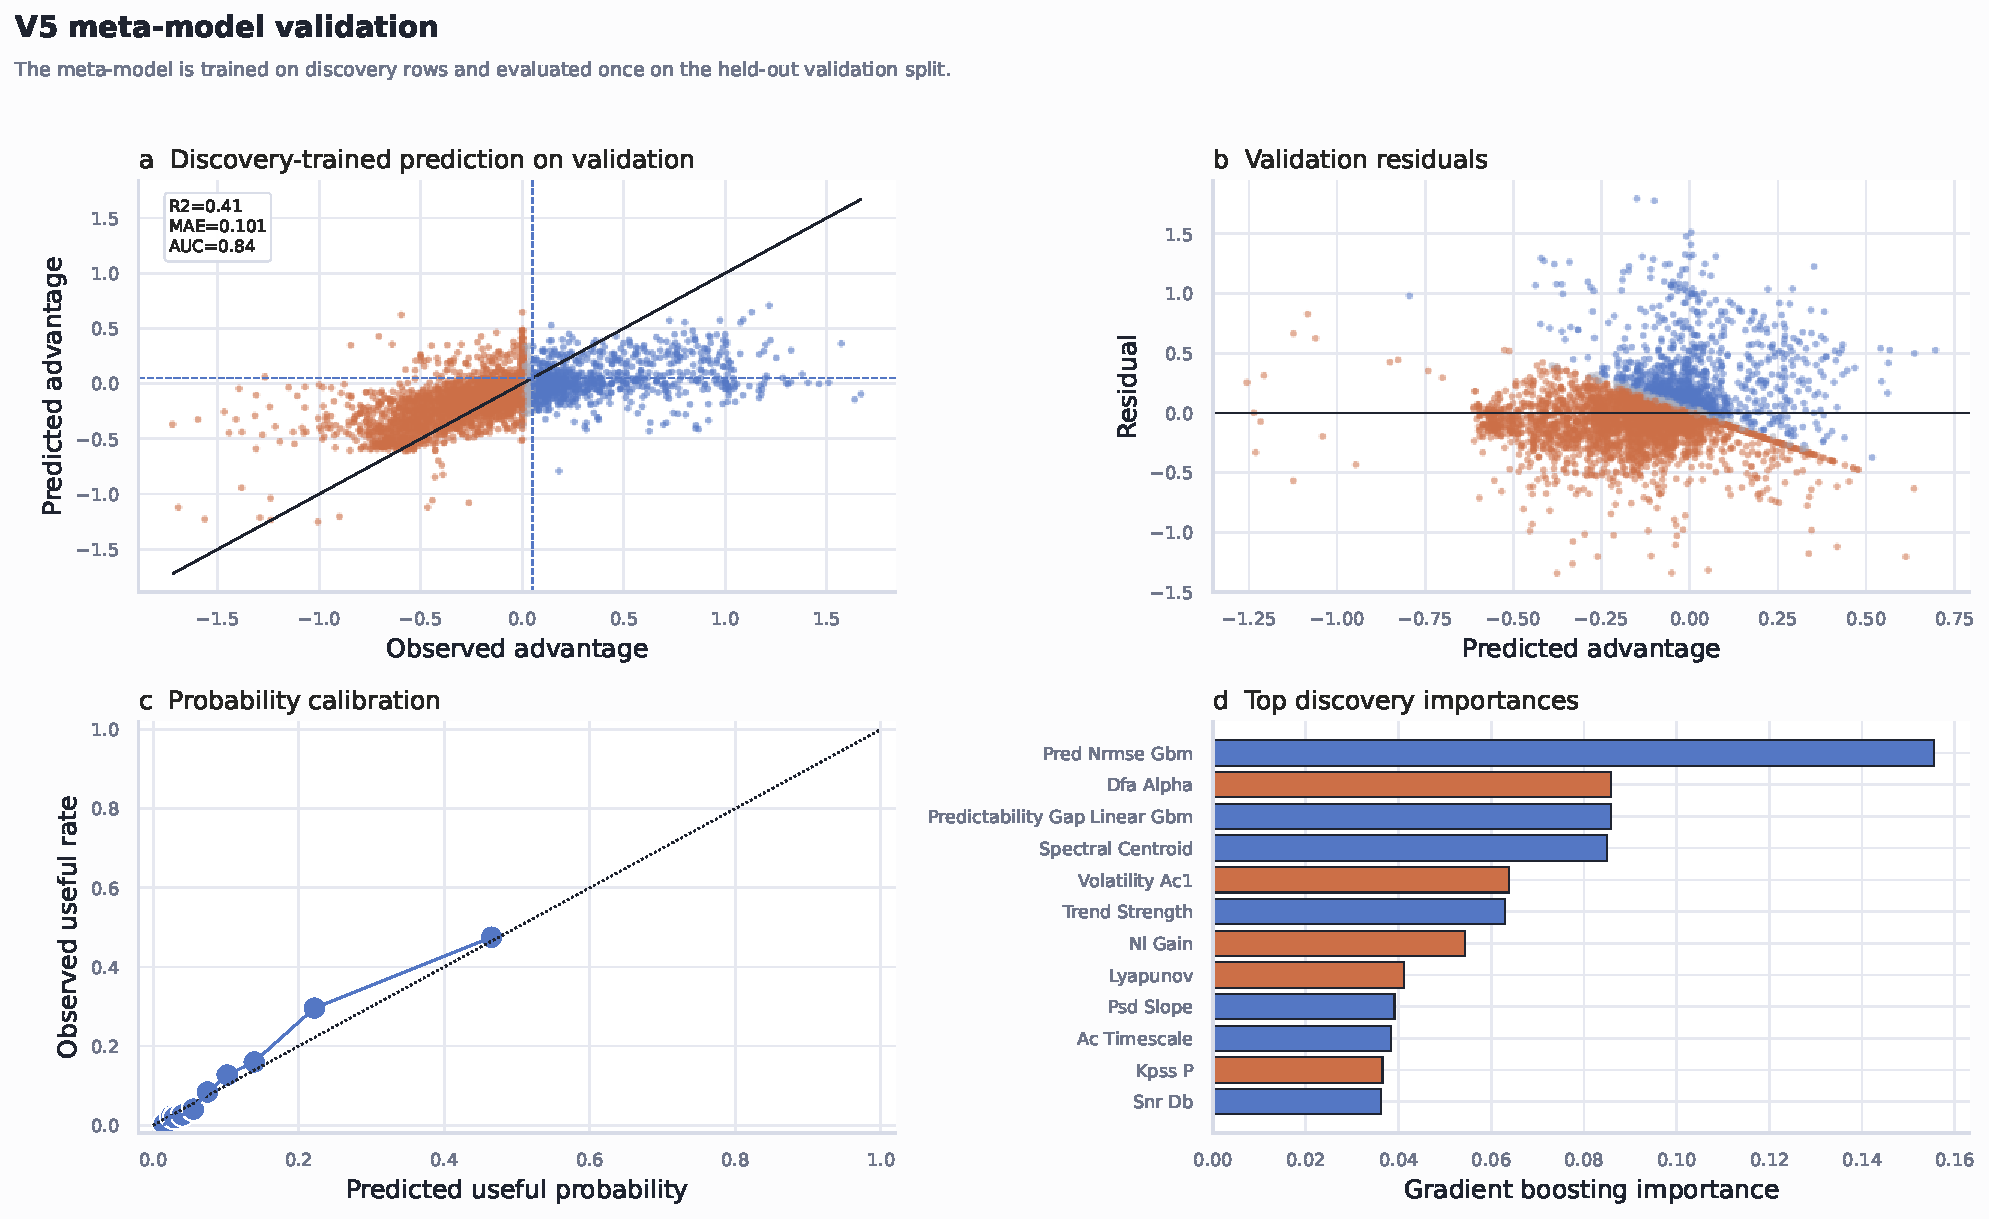
\includegraphics[width=\textwidth]{meta-model-validation.pdf}
    \caption{Meta-model validation. The model is trained on discovery rows and evaluated once on held-out validation rows. The panels show predicted versus observed advantage, probability calibration, and discovery-trained feature importance.}
    \label{fig:meta-model}
\end{figure*}

The discovery-trained meta-model predicts validation advantage with \(R^2=0.407\) and MAE 0.101. For the binary useful label, it obtains ROC-AUC 0.836 and PR-AUC 0.431 against a 12.5\% base rate. This is strong enough for triage: the model ranks held-out datasets by QRC usefulness from measured descriptors, before running QRC on those rows.

The important descriptors are not a single axis. Top features include GBM predictability, scaling exponent, predictability-gap structure, spectral centroid, volatility autocorrelation, trend strength, nonlinear-gain contrast, Lyapunov estimate, spectral slope, autocorrelation time, stationarity signal, and SNR. The signs are mixed because the map is interaction-driven: the same descriptor can be favorable in one region and unfavorable in another.

\subsection{Slow, stateful regimes are most favorable}

\begin{figure}[!t]
    \centering
    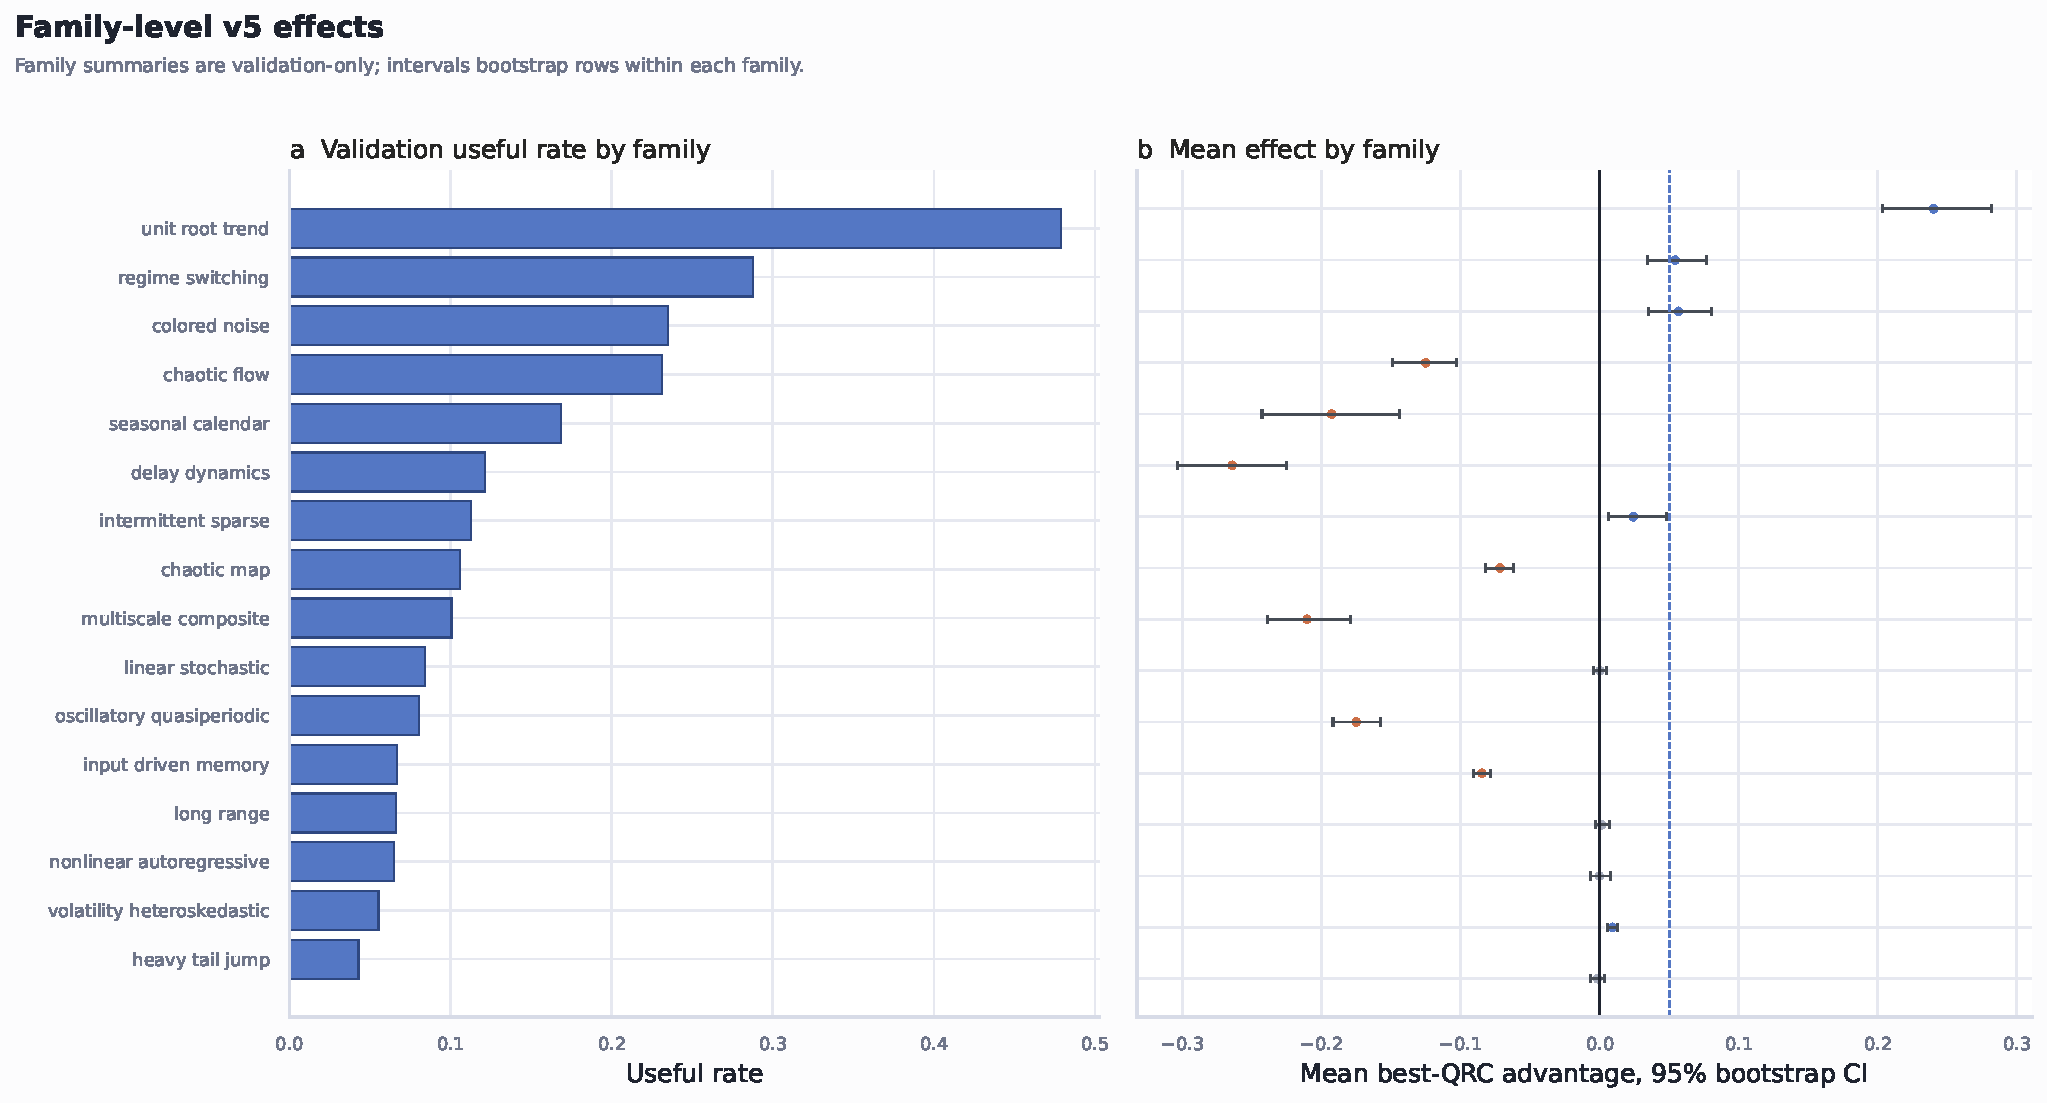
\includegraphics[width=\columnwidth]{family-effects.pdf}
    \caption{Validation family effects. Drifting-trend, regime-switching, and colored-noise families have the clearest positive mean effects. Several families contain useful pockets despite negative family-average advantage, showing why row-level triage is needed.}
    \label{fig:family-effects}
\end{figure}

\autoref{fig:family-effects} and \autoref{tab:family-top} summarize the family-level structure. The strongest family is the drifting-trend family, with 47.9\% useful rate, 51.8\% win rate, and mean advantage \(+0.240\) with 95\% bootstrap interval \([+0.203,+0.282]\). Regime switching and colored noise also have positive mean effects and useful rates above 23\%. Intermittent sparse and linear stochastic families have high win rates but small mean effects, indicating many near-ties rather than large QRC gains.

\begin{table}[!t]
\centering
\caption{Top validation families by useful QRC rate.}
\label{tab:family-top}
\scriptsize
\setlength{\tabcolsep}{2.6pt}
\renewcommand{\arraystretch}{1.02}
\begin{tabular}{lrrrr}
\toprule
Family & \(n\) & Useful & Win & Mean adv. \\
\midrule
Drifting trend & 353 & 47.9 & 51.8 & +0.240 \\
Regime switching & 313 & 28.8 & 48.2 & +0.054 \\
Colored noise & 315 & 23.5 & 48.6 & +0.057 \\
Chaotic flow & 1137 & 23.1 & 29.6 & -0.125 \\
Seasonal/calendar & 255 & 16.9 & 25.9 & -0.193 \\
Delay dynamics & 231 & 12.1 & 15.6 & -0.264 \\
Intermittent sparse & 142 & 11.3 & 53.5 & +0.024 \\
Chaotic map & 2056 & 10.6 & 28.5 & -0.072 \\
\bottomrule
\end{tabular}
\end{table}

The strongest extracted validation rule pocket is also interpretable. Rows with high trend strength and low spectral centroid form a pocket of 420 validation datasets with 47.4\% useful rate and mean advantage \(+0.209\). This is not a mechanism proof. It is a compact triage rule: slow, trend-heavy, low-frequency structure is a high-priority region for testing QRC.

\subsection{The map is robust to feature choices}

The feature-set robustness table supports the anti-circularity claim. The full 30-feature map reaches validation ROC-AUC 0.836 and PR-AUC 0.431. Using only the original 20 core descriptors gives ROC-AUC 0.828 and PR-AUC 0.423. Removing direct predictability proxies gives ROC-AUC 0.834 and PR-AUC 0.432. Restricting to persistence, spectrum, volatility, and nonstationarity gives ROC-AUC 0.827 and PR-AUC 0.409. Thus the atlas is not simply rediscovering which baseline already won.

\begin{table}[!t]
\centering
\caption{Validation robustness of meta-model feature sets.}
\label{tab:feature-robustness}
\scriptsize
\setlength{\tabcolsep}{3.2pt}
\renewcommand{\arraystretch}{1.04}
\begin{tabular}{lrrr}
\toprule
Feature set & \(R^2\) & ROC & PR \\
\midrule
Full 30 descriptors & .407 & .836 & .431 \\
Original 20 core & .383 & .828 & .423 \\
No predictability proxies & .392 & .834 & .432 \\
No chaos/nonlinear/complexity & .384 & .831 & .430 \\
Persistence/spectrum/drift & .364 & .827 & .409 \\
Chaos/nonlinear/complexity only & .324 & .798 & .359 \\
\bottomrule
\end{tabular}
\end{table}

Threshold robustness leads to the same conclusion. The validation useful rate is 35.4\% at threshold 0, 17.5\% at 0.025, 12.5\% at 0.05, and 8.5\% at 0.1. Stricter thresholds make QRC advantage rarer, but they do not erase the slow-stateful pocket.

\subsection{What the triage map means}

The practical output is a screening rule, not a universal deployment rule. A practitioner can measure the 30 descriptors, locate the dataset in property space, and decide whether QRC evaluation is worth the extra cost. High predicted usefulness does not guarantee a QRC win; it identifies a region where the empirical evidence says QRC deserves testing. Low predicted usefulness is equally useful: it says the ESN is likely to be the better default unless there is a separate hardware, physical, or scientific reason to test a quantum reservoir.


\section{Conclusion}
\label{sec:conclusion}
We introduced a dataset-regime benchmark for empirical quantum reservoir advantage against echo state networks. The main result is deliberately two-sided. ESNs remain the stronger default: QRC does not win on average under the globally frozen protocol. At the same time, QRC wins are reproducible, structured, and predictable from measured dataset properties. The strongest and most likely QRC-usefulness regime in the current evidence is slow, stateful forecasting: drifting trends, regime changes, persistent low-frequency structure, long memory, and temporally correlated fluctuations.

The benchmark therefore turns QRC selection into a measurable triage problem. Practitioners need not ask whether QRC is universally better. They can profile a dataset, compare it with the atlas, and decide whether quantum-reservoir evaluation is worth the cost relative to a strong ESN baseline. This is the practical meaning of quantum reservoir advantage in this paper, and the released code exposes it as a CSV-based triage tool for new univariate forecasting datasets.

The next scientific step is mechanistic. The atlas identifies where QRC helps; it does not yet prove why. Follow-up work should measure reservoir-state memory kernels, latent-state recoverability, phase/coupling/dissipation ablations, and matched long-memory ESN controls in the high-usefulness pockets identified here. Those studies can test whether the observed slow-structure regimes arise from genuinely quantum feature dynamics or from a broader reservoir-memory design principle.

The strongest claim supported now is therefore not universal quantum advantage. It is a regime-map claim: empirical quantum reservoir advantage is selective, measurable, and predictable under a fair frozen comparison against an ESN. That claim is useful even when QRC loses on average, because it gives the field a concrete way to decide where QRC evidence should be concentrated next.


\section*{Reproducibility and Claim Boundary}
The artifact tree separates the protocol, labels, analysis tables, figures, and paper draft. The main v5 evidence used here is stored under \texttt{results\_frontier\_v5\_discovery/}, \texttt{results\_frontier\_v5\_validation/}, and \texttt{results\_v5\_publication/}. The title uses ``quantum reservoir advantage'' in the empirical benchmark sense: lower forecasting error for a frozen QRC variant than for a frozen feature-matched ESN under the declared protocol. We do not claim computational quantum advantage, broad average QRC superiority, or a proven coupling/interference mechanism.

\bibliographystyle{IEEEtranDoi}
\bibliography{references}
\end{document}
